\documentclass[letterpaper, 10pt,titlepage]{article}

\usepackage[utf8]{inputenc}
\usepackage [english]{babel}
\usepackage [autostyle, english = american]{csquotes}
\usepackage{graphicx}                                        
\usepackage{amssymb}                                         
\usepackage{amsmath}                                         
\usepackage{amsthm}                                          
\usepackage{alltt}                                           
\usepackage{float}
\usepackage{url}
\newcommand\tab[1][1cm]{\hspace*{#1}}
\setlength{\parindent}{0em}
\setlength{\parskip}{1em}
\usepackage{pst-gantt}
\usepackage[letterpaper, margin=0.75in]{geometry}
\usepackage{balance}
\usepackage[TABBOTCAP, tight]{subfigure}
\usepackage{enumitem}
\usepackage{pstricks, pst-node}
\usepackage{hyperref}
\hypersetup{
  colorlinks = true,
  linkcolor  = black
}
\usepackage{listings}
\usepackage{color}
 
\definecolor{codegreen}{rgb}{0,0.6,0}
\definecolor{codegray}{rgb}{0.5,0.5,0.5}
\definecolor{codepurple}{rgb}{0.58,0,0.82}
\definecolor{backcolour}{rgb}{0.95,0.95,0.92}
 
\lstdefinestyle{mystyle}{
    backgroundcolor=\color{backcolour},   
    commentstyle=\color{codegreen},
    keywordstyle=\color{magenta},
    numberstyle=\tiny\color{codegray},
    stringstyle=\color{codepurple},
    basicstyle=\footnotesize,
    breakatwhitespace=false,         
    breaklines=true,                 
    captionpos=b,                    
    keepspaces=true,                 
    numbers=left,                    
    numbersep=5pt,                  
    showspaces=false,                
    showstringspaces=false,
    showtabs=false,                  
    tabsize=2
}
 
\lstset{style=mystyle}
\usepackage{minted}




\setcounter{secnumdepth}{4}
\def\name{Jiawei Liu}

\hypersetup{
  colorlinks = true,
  urlcolor = black,
  pdfauthor = {\name},
  pdfkeywords = {Problem Statement},
  pdftitle = {Capstone Project},
  pdfsubject = {Capstone Project},
  pdfpagemode = UseNone
}



\begin{document}

\begin{titlepage}
\begin{center}
    \Huge
    \textbf{Winter Midterm Progress Report}\\
    \textbf{Capstone Project}\\
    \vspace{1.0cm}
    \large
    Developers: Charles Henninger, Duncan Millard, Jiawei Liu\\
    Sponsor: Nancy Hildebrandt\\
    \vspace{1.5cm}
    \large
    Instructor: D. Kevin McGrath\\

    \large
    CS 462, Winter 2017, Oregon State University\\    

    \vspace{3.2cm}

    \large
    \underline{Abstract}\\
    \vspace{0.3cm}
    \end{center}
    \large

    \tab The Santiam wagon trail is historic trail located in the Willamette National Forest. The local ranger stations wish to have a mobile app that is capable of taking users on a tour of the wagon trail without needing a connection to the internet. The mobile application come in two forms: one developed for the Android mobile platform, and the other developed for the iOS mobile platform. While these two forms of the mobile application will be developed separately, they will be using the same methods of providing a tour to the user. The mobile application will render a map using a pre-downloaded map tile file and place waypoints onto the map that will be related to relevant information, in the form of videos and text files, about that area of the map. In order to achieve this functionality without internet access, we will rely on pre-downloaded content packs that will contain the map tiles, videos, text files, and waypoint information. These content packages will be created by staff of the local ranger stations, and uploaded via a website that will be developed along with the mobile app. Our team will divide these three larger sections of this project (the Android application, iOS application, and the Web Control panel/backend engineering) between the team members as follows: Android application development: Charles Henninger, Web Control panel/backend engineering: Duncan Millard, iOS application development: Jiawei Liu. This document outlines the possible technologies that will be used to address problems in each of these three major development sections, written by the team member heading each of the sections.
    
    \vspace{0.8cm}
    \vfill
    
\begin{center}    
    Feb 17, 2016

\end{center}
\end{titlepage}


\tableofcontents
\newpage



\section{Introduction}
\subsection{Team number and project name}
We are group \#43, and project name is Santiam Wagon Trail Mobile App.


\subsection{Team members and role in the project}
Jiawei Liu: The role as a UI designer which work on iOS UI, Web Control Panel UI, and Remote API Interactions. \\
Charles Henninger: Android UI Design and Functionality, Map Rendering, Android Remote API Interactions\\
Duncan Millard: Web Control Panel functionality, Inter-App framework


\vspace{0.3cm}




\section{Jiawei Liu's Section}

\subsection{iOS App Development}
This project is going to develop iOS and Android map, then offer a web control panel to manage waypoints. In detail, this project will include a mobile application (iOS and Android), the Trail Companion, that will work with custom content packages downloaded in the app. A website will be included for administrators to upload content packages to a server where the application then request and download the packages. The mobile application will provide the user with an interactive map of an area, the user’s location, and waypoints on within the area containing information about the park. This application will require no Internet access after downloading the content packages and application itself.
 
Currently, I am working on the iOS app for our project. I finished the basic UI and include all setting options in the page such as silent mode, app version, credits and help page. As screenshots show, the home page will be “My Tours” and display the map, waypoints and user’s location. Then, there are four subpages when the user click menu button, which are My Tours, Discover, Setting and Help. Now the setting page and help page are ready for use.
 
The next step of iOS app development is read waypoints and download the content package from our server. In the rest of this term, I will mainly work on the connection between server and iOS app. For example, read the available region, show waypoints on the map, and load detail description from the content package.
 
During the iOS app development, the major problem is nobody familiar with iOS development, and OSU doesn’t teach iOS development. And then, iOS using Swift to develop apps, so I need to learn a new language to develop the iOS app. Our group decides to use Android style slider menu as our app’s UI, but this is not the default iOS UI, I will include extra style file to achieve it. In addition, Xcode doesn’t like Android Studio, it only works on Mac OS system. For the map, since most map providers charge for using offline map, we also did some research for the map provider to avoid charging.
 
For solving above problems, I begin to learn how to develop iOS app on the Internet. There are some good tutorials on YouTube and Apple website to help me begin the project. Since I can find some useful tutorials on the Internet, so it solved the problem that nobody familiar with iOS development. For learning swift, I found a website called “runoob.com”, this website provides a helpful tutorial for swift, I learn the basic knowledge of swift programming during the winter break. For the UI, since Xcode didn’t include this UI template, so I google how to design slide bar in iOS. Fortunately, I found a great tutorial about how to create a slider menu on iOS, which is “ashishkakkad.com”. Then I use this tutorial as the template to develop our project. Since I am the only person that owns a Mac device in our group, I decide to work on iOS app development. For the map provider, since Mapbox can provide free offline map and customized map. We choose Mapbox as the map provider and the default map framework.
 
For solving above problems, I start to learn how to develop iOS app on the Internet. There are some good tutorials on YouTube and Apple website to help me begin the project. Since I can find some useful tutorials on the Internet, so it solved the problem that nobody familiar with iOS development. For learning swift, I found a website called “runoob.com”, this website provides a good tutorial for swift, I learn the basic knowledge of swift programming during the winter break. For the UI, since Xcode didn’t include this UI template, so I google how to design slide bar in iOS. Fortunately, I found a great tutorial about how to create slide menu on iOS, which is “ashishkakkad.com”. then I use this tutorial as the template to develop our project. Since I am the only person that own a Mac device in our group, I decide to work on iOS app development. For the map provide, Since Mapbox can provide free offline map and customized map. We choose Mapbox as the map provider and default map framework. In addition, Mapbox has a detailed tutorial to teach me how to include the map in the iOS app and display waypoints.

According to thefreedictionary.com, the definition of experimental design is “research design that eliminates all factors that influence outcome except for the cause being studied (independent variable). All other factors are controlled by randomization, investigator-controlled manipulation of the independent variable, and control of the study situation by the investigator, including the use of control groups. [1]” In my opinion, experimental design is useful for our project, it can improve our design and provide a more comfortable user experience. For example, I can design an experiment to test user map preference in many ways. I can download couples of maps app such as Google Map, Here Map, and Open Street Map. We can observe users’ habit and summary their preference. Then we can optimize our app UI and provide a better user experience.
 
For the interface design, we discussed the UI design as a group and our group member Charles did a great app UI paper prototypes, then uploaded to our group GitHub. We use this paper prototype as the reference to develop our project. I hope users are going to click the waypoint and understand how to visit the waypoint when the first time they use this app. In addition, Since I used the Android style slider menu, it is popular in Android but not in iOS, I hope users can click the menu button to check more features.
 
For the screenshots, I have six screenshots, which are home page, slider menu, setting page, help page, Xcode and Storyboard at the bottom of report. 


\subsection{Swift Code for Slider Menu}
\begin{minted}{swift}
import UIKit

protocol SlideMenuDelegate {
    func slideMenuItemSelectedAtIndex(_ index : Int32)
}

class MenuViewController: UIViewController, UITableViewDataSource, UITableViewDelegate {

    @IBOutlet var tblMenuOptions : UITableView!
    
    @IBOutlet var btnCloseMenuOverlay : UIButton!

    var arrayMenuOptions = [Dictionary<String,String>]()
    var btnMenu : UIButton!
    var delegate : SlideMenuDelegate?
    
    override func viewDidLoad() {
        super.viewDidLoad()
        tblMenuOptions.tableFooterView = UIView()
        // Do any additional setup after loading the view.
    }
    
    override func didReceiveMemoryWarning() {
        super.didReceiveMemoryWarning()
        // Dispose of any resources that can be recreated.
    }
    
    override func viewWillAppear(_ animated: Bool) {
        super.viewWillAppear(animated)
        updateArrayMenuOptions()
    }
    
    func updateArrayMenuOptions(){
        arrayMenuOptions.append(["title":"My Tours", "icon":"HomeIcon"])
        arrayMenuOptions.append(["title":"Discover", "icon":"PlayIcon"])
        arrayMenuOptions.append(["title":"Setting", "icon":"SettingIcon"])
        arrayMenuOptions.append(["title":"Help", "icon":"HelpIcon"])
        
        tblMenuOptions.reloadData()
    }
    
    @IBAction func onCloseMenuClick(_ button:UIButton!){
        btnMenu.tag = 0
        
        if (self.delegate != nil) {
            var index = Int32(button.tag)
            if(button == self.btnCloseMenuOverlay){
                index = -1
            }
            delegate?.slideMenuItemSelectedAtIndex(index)
        }
        
        UIView.animate(withDuration: 0.3, animations: { () -> Void in
            self.view.frame = CGRect(x: -UIScreen.main.bounds.size.width, y: 0, width: UIScreen.main.bounds.size.width,height: UIScreen.main.bounds.size.height)
            self.view.layoutIfNeeded()
            self.view.backgroundColor = UIColor.clear
            }, completion: { (finished) -> Void in
                self.view.removeFromSuperview()
                self.removeFromParentViewController()
        })
    }
    
    func tableView(_ tableView: UITableView, cellForRowAt indexPath: IndexPath) -> UITableViewCell {
        let cell : UITableViewCell = tableView.dequeueReusableCell(withIdentifier: "cellMenu")!
        
        cell.selectionStyle = UITableViewCellSelectionStyle.none
        cell.layoutMargins = UIEdgeInsets.zero
        cell.preservesSuperviewLayoutMargins = false
        cell.backgroundColor = UIColor.clear
        
        let lblTitle : UILabel = cell.contentView.viewWithTag(101) as! UILabel
        let imgIcon : UIImageView = cell.contentView.viewWithTag(100) as! UIImageView
        
        imgIcon.image = UIImage(named: arrayMenuOptions[indexPath.row]["icon"]!)
        lblTitle.text = arrayMenuOptions[indexPath.row]["title"]!
        
        return cell
    }
    
    func tableView(_ tableView: UITableView, didSelectRowAt indexPath: IndexPath) {
        let btn = UIButton(type: UIButtonType.custom)
        btn.tag = indexPath.row
        self.onCloseMenuClick(btn)
    }
    
    func tableView(_ tableView: UITableView, numberOfRowsInSection section: Int) -> Int {
        return arrayMenuOptions.count
    }
    
    func numberOfSections(in tableView: UITableView) -> Int {
        return 1;
    }
}

\end{minted}


\vspace{0.5cm}


\section{Charles Henninger's Section}
XXXXXXXXXXXXXXXX

\vspace{0.5cm}

\section{Duncan Millard's Section}

balabalabala







\newpage %add references at here
\begin{thebibliography}{9}

\bibitem{1} 
"thefreedictionary," \textit{thefreedictionary}. [Online]. \\Available:
\texttt{http://medical-dictionary.thefreedictionary.com/experimental+design} [Accessed: 16-Feb-2017].
%%

\end{thebibliography}




\newpage
\section{Screenshots}

\begin{figure}[ht]
    \centering
    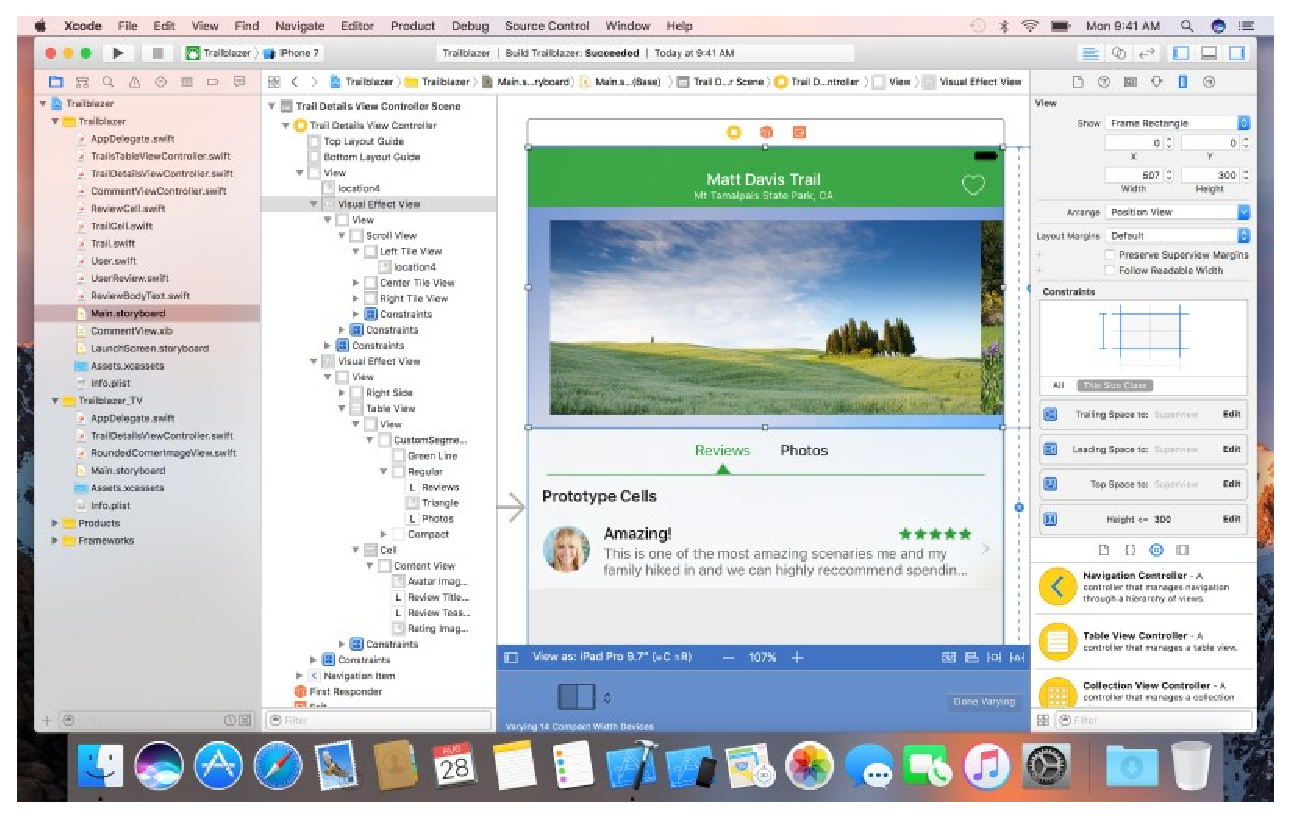
\includegraphics[scale=0.5]{j1}
    \caption{My Tours}
    \label{jiawei1}
\end{figure}

\begin{figure}[ht]
    \centering
    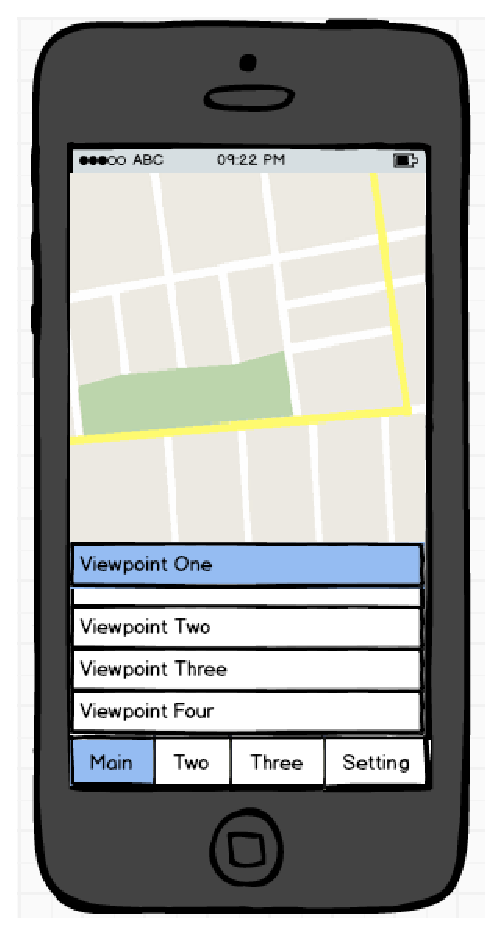
\includegraphics[scale=0.5]{j2}
    \caption{Slider Menu}
    \label{jiawei2}
\end{figure}

\begin{figure}[ht]
    \centering
    \includegraphics[scale=0.5]{j3}
    \caption{Setting}
    \label{jiawei3}
\end{figure}

\begin{figure}[ht]
    \centering
    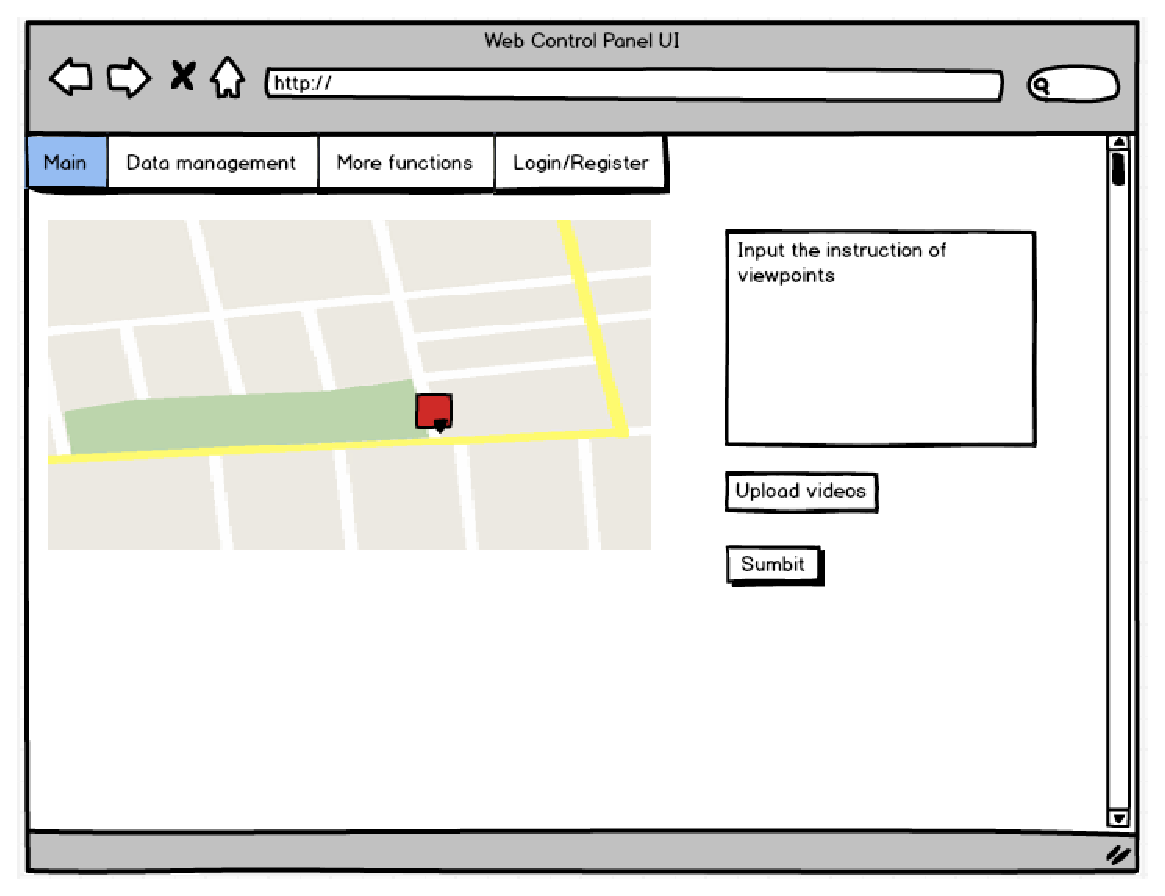
\includegraphics[scale=0.5]{j4}
    \caption{Help}
    \label{jiawei4}
\end{figure}

\begin{figure}[ht]
    \centering
    \includegraphics[width=0.8\textwidth]{j5}
    \caption{Xcode}
    \label{jiawei5}
\end{figure}

\begin{figure}[ht]
    \centering
    \includegraphics[scale=0.5]{j6}
    \caption{Storyboard}
    \label{jiawei6}
\end{figure}










\end{document}
